\chapter{TỔNG QUAN}
    \section{Tìm hiểu về AGVs}
    \subsection{Tổng quan về AGVs}
    \hspace*{0.6cm} AGVs (Automated Guided Vehicles) hay còn gọi là hệ thống robot tự hành, là các robot có khả năng tự lái, sử dụng động cơ điện,
    tích hợp điều khiển trong một phần mềm hệ điều hành chính để có khả năng lập trình lựa chọn đường đi, điểm đến và tránh va chạm, 
    có nhiệm vụ chuyên chở, xếp dỡ hàng hóa, vật liệu trong các nhà máy, kho xưởng, v.v.
    \subsection{Phân loại}
    \hspace*{0.6cm} Dựa theo chức năng và hình dáng cấu tạo, AGVs được chia thành các loại phổ biến:
    \begin{itemize}
        \item Robot di động chui gầm (Latent Mobile Robot): robot chui xuống dưới pallets để nâng toàn bộ pallets lên, đưa đến đích và hạ xuống.
            \begin{figure}[H]
                \centering
                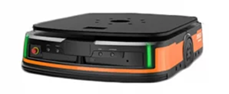
\includegraphics[width=0.5\textwidth]{pictures/chapter1/chapter1_pic_1.png}
                \caption{Latent Mobile Robot}
                \label{chap1_pic1}
            \end{figure}
        \item Robot di động băng chuyền (Conveyer Mobile Robot): robot được thiết kế để tiếp nối chuyển giao với các dây chuyền sản xuất.
            \begin{figure}[H]
                \centering
                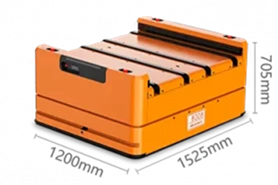
\includegraphics[width=0.45\textwidth]{pictures/chapter1/chapter1_pic_2.png}
                \caption{Conveyer Mobile Robot}
                \label{chap1_pic2}
            \end{figure}
        \item Robot di động nâng hạ (Forklift Mobile Robot): Thực hiện việc nâng hạ hàng, đưa lên những robot khác hoặc các line sản xuất.
            \begin{figure}[H]
                \centering
                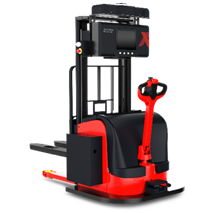
\includegraphics[width=0.4\textwidth]{pictures/chapter1/chapter1_pic_3.png}
                \caption{Forklift Mobile Robot}
                \label{chap1_pic3}
            \end{figure}
        \item Robot di động tải nặng (Heavy-duty mobile robot): có kích thước lớn và chịu tải tốt, dùng trong nâng ô tô và các ứng dụng khác đòi hỏi chịu tải cao.
            \begin{figure}[H]
                \centering
                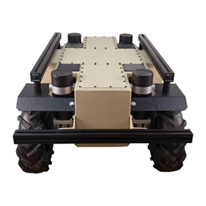
\includegraphics[width=0.35\textwidth]{pictures/chapter1/chapter1_pic_4.png}
                \caption{Heavy-duty Mobile Robot}
                \label{chap1_pic4}
            \end{figure}
    \end{itemize}

    \subsection{Các kỹ thuật điều khiển và dẫn hướng AGVs}
    \hspace*{0.6cm} Những thiết bị điều khiển hệ thống của AGV được chia làm 2 loại: hệ thống điều khiển cố định và hệ thống điều khiển ngoại vi. 
    Nhiệm vụ của hệ thống điều khiển cố định là quản lý vận chuyển, tối ưu hóa hành trình và giao tiếp với các hệ thống khác. Hệ thống điều khiển
    ngoại vi có nhiệm vụ quản lý các thiết bị trên xe như thiết bị nâng hạ, thiết bị sạc. \\
    \hspace*{0.6cm} Các kỹ thuật điều hướng cho AGVs:
    \begin{itemize}
        \item Dẫn hướng bởi dây điện (Wire guidance navigation): Sử dụng những dây điện mang tần số thấp chôn dưới sàn và có thể được phát 
        hiện bằng cảm biến điện từ gắn trên AGVs, phương pháp này còn gọi là điều hướng điện từ.
            \begin{figure}[H]
                \begin{subfigure}{0.5\textwidth}
                \centering
                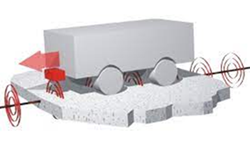
\includegraphics[width=0.6\linewidth, right]{pictures/chapter1/chapter1_pic_5a.png} 
                \label{chap1_pic5a}
                \end{subfigure}
                \begin{subfigure}{0.5\textwidth}
                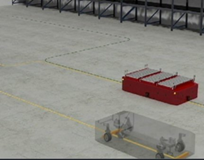
\includegraphics[width=0.5\linewidth]{pictures/chapter1/chapter1_pic_5b.png}
                \label{chap1_pic5b}
                \end{subfigure}
                \caption{AGVs dẫn hướng bằng dây}
                \label{chap1_pic5}
            \end{figure}
        \begin{itemize}[label=\textendash]
            \item Ưu điểm: Độ chính xác và ổn định cao, không bị ảnh hưởng bởi nhiễu ánh sáng, chi phí cảm biến thấp.
            \item Nhược điểm: Khó bảo trì, sửa chữa, không phù hợp trong môi trường đòi hỏi linh hoạt và điều kiện môi trường thay đổi. 
        \end{itemize}
        \item Dẫn hướng bằng băng từ (Magnetic tape guidance navigation): Nguyên lý tương tự như điều hướng bằng dây nhưng sử dụng băng
        từ đặt trên mặt đất. Phương pháp trên tốn kém ít chi phí hơn trong lắp đặt nhưng đồng thời cũng dễ bị hư hại, phải mất thêm chi phí bảo trì, sửa chữa.
            \begin{figure}[H]
                \begin{subfigure}{0.5\textwidth}
                \centering
                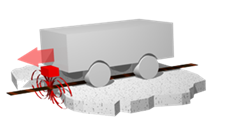
\includegraphics[width=0.6\linewidth, right]{pictures/chapter1/chapter1_pic_6a.png} 
                \label{chap1_pic6a}
                \end{subfigure}
                \begin{subfigure}{0.7\textwidth}
                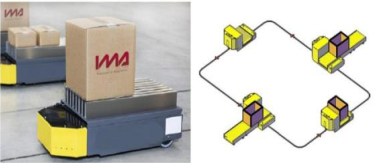
\includegraphics[width=0.7\linewidth]{pictures/chapter1/chapter1_pic_6b.png}
                \label{chap1_pic6b}
                \end{subfigure}
                \caption{AGVs dẫn hướng bằng băng từ}
                \label{chap1_pic6}
            \end{figure}
        \begin{itemize}[label=\textendash]
            \item Ưu điểm: Di chuyển chính xác trên băng dẫn, dễ dàng thay đổi đường đi, chi phí
            thấp, không bị ảnh hưởng ánh sáng, bụi bẩn
            \item Nhược điểm: Băng dán dễ bị hỏng, phải được bảo trì thường xuyên, không phù
            hợp với các dự án có yêu cầu lộ trình phức tạp, dễ bị ảnh hưởng bởi nhiễu điện từ. 
        \end{itemize} 
        \item Dẫn hướng bằng cảm biến quang học (Optical track guidance navigation): Tương tự với dẫn hướng bằng băng từ
        bằng cách bố trí những đường màu trên đường đi. Phương pháp này đòi hỏi máy ảnh và chức năng xử lí hình ảnh để nhận diện đường đi. Cũng yêu cầu bảo trì 
        nhưng ít tốn kém hơn bởi khả năng thích ứng cao với nhiễu điện từ. 
            \begin{figure}[H]
                \begin{subfigure}{0.5\textwidth}
                \centering
                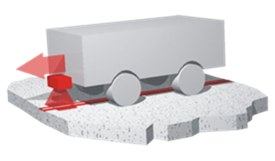
\includegraphics[width=0.6\linewidth, right]{pictures/chapter1/chapter1_pic_7a.png} 
                \label{chap1_pic7a}
                \end{subfigure}
                \begin{subfigure}{0.7\textwidth}
                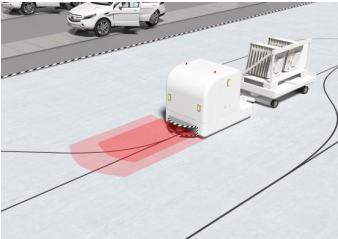
\includegraphics[width=0.5\linewidth]{pictures/chapter1/chapter1_pic_7b.png}
                \label{chap1_pic7b}
                \end{subfigure}
                \caption{AGVs dẫn hướng bằng cảm biến quang học}
                \label{chap1_pic7}
            \end{figure}
        \begin{itemize}[label=\textendash]
            \item Ưu điểm: Lắp đặt nhanh, dễ thực hiện, thay đổi điều chỉnh lại dễ dàng, chi phí
            thấp, dễ thực hiện.
            \item Nhược điểm: Các vạch dẫn trên bề mặt đường đi dễ bị nhiễm bẩn, hư hại bởi các yếu
            tố ngoại quan. Dễ bị ảnh hưởng bởi điều kiện ánh sáng.
        \end{itemize}
        \item Dẫn hướng bằng laser dẫn đường (Laser target navigation): Robot sử dụng bộ thu phát Laser và đo khoảng cách đến các điểm cố định (tấm
        gương) được lắp đặt trong nhà máy từ đó xác định được vị trí trong nhà máy và đường
        di chuyển.
            \begin{figure}[H]
                \centering
                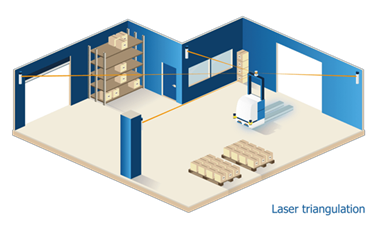
\includegraphics[width=0.5\textwidth]{pictures/chapter1/chapter1_pic_8a.png}
                \caption{AGVs dẫn hướng bằng cảm biến laser}
                \label{chap1_pic8}
            \end{figure}
        \begin{itemize}[label=\textendash]
            \item Ưu điểm: Độ chính xác trong định vị cao, tốc độ nhanh.
            \item Nhược điểm: Độ chính xác và hiệu quả giảm đi nếu các tấm phản chiếu bị che mất. 
            Do đó phương pháp này còn đòi hỏi điều kiện làm việc của môi trường.
        \end{itemize}
        \item Dẫn hướng bằng camera (Camera-based navigation): Robot sử dụng Camera để thu thập hình ảnh môi trường xung quanh và từ đó xác
        định vị trí và đường di chuyển tiếp theo.
            \begin{figure}[H]
                \centering
                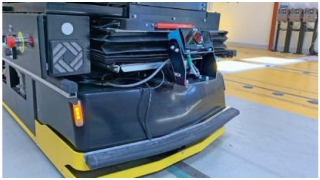
\includegraphics[width=0.5\textwidth]{pictures/chapter1/chapter1_pic_9.png}
                \caption{AGVs dẫn hướng bằng camera}
                \label{chap1_pic9}
            \end{figure}
        \begin{itemize}[label=\textendash]
            \item Ưu điểm: Độ linh hoạt cao, phù hợp với các môi trường có điều kiện làm việc phức tạp, thay đổi liên tục.
            \item Nhược điểm: Công nghệ phức tạp, đòi hỏi phải xử lý lượng dữ liệu lớn, thường chỉ
            được sử dụng cho một số ứng dụng đặc thù.
        \end{itemize}   
    \end{itemize} 

    \section{Sơ lược về robot dò line}
    \hspace*{0.6cm} Robot dò line (Line following Robot) là một dạng robot di động (mobile robot) di
    chuyển bằng bánh xe. Robot sẽ di chuyển bám theo các đường line được kẻ/vẽ/dán trên
    mặt đất. Quỹ đạo di chuyển của robot phụ thuộc vào sa bản của hệ thống các đường line
    được kẻ/vẽ/dán sẵn. Một robot dò line gồm các yếu tố: sơ đồ nguyên lý, loại cảm biến,
    động cơ, cấu trúc điều khiển. \\
    \hspace*{0.6cm} Hiện nay, có rất nhiều kết cấu cơ khí được thiết kế để cải thiện khả năng di chuyển
    của robot dò line như đáp ứng tốc độ, độ chính xác bám line,\dots. Các kết cấu hiện nay
    phổ biến là: cấu trúc hai bánh, ba bánh, bốn bánh, bánh xích, \dots \\
    \hspace*{0.6cm} Trong phạm vi của đề tài, nhóm hướng đến thiết kế robot dò line bám đường và
    có khả năng nhận diện được màu sắc của kiện hàng được đặt lên xe tại khu vực tải hàng, từ đó phân phối hàng hóa đến vị trí kết thúc theo quỹ đạo có màu sắc tương ứng với màu sắc của gói hàng.


    \section{Các sản phẩm ở trong và ngoài nước}
    \subsection{Robot Zumo Slim}
    \hspace*{0.6cm} Robot Zumo Slim là robot của anh Zeremy trong cuộc thi LVBots line following.
    \begin{itemize}
        \item Sơ đồ nguyên lý cơ khí:
        % image 10
        \item Các thành phần của robot:
            \begin{itemize}[label=\textendash]
                \item Động cơ DC có encoder, có hộp số tỉ lệ 10:1.
                \item Cảm biến: Cảm biến line và cảm biến tiệm cận được gắn ở đầu xe.
                \item Vi điều khiển: Zumo's ATmega32U4.
                \item Bánh xe: Sử dụng 3 bánh, 2 bánh chủ động phía sau và 1 bánh bị động tự lựa phía trước.
            \end{itemize}
    \end{itemize}

    \subsection{Robot Pinto}
    \hspace*{0.6cm} Robot Pinto là robot từng tham gia trong cuộc thi LVBots line following 2015 và 2018.
    \begin{itemize}
        \item Sơ đồ nguyên lý cơ khí:
        %image 11
        \item Các thành phần của robot:
            \begin{itemize}[label=\textendash]
                \item Động cơ: 2 động cơ DC có tích hợp Encoder, sử dụng driver VNH5019.
                \item Cảm biến: 8 cảm biến hồng ngoại Pololu QTR-8RC, được đặt thành dãy ở đầu xe.
                \item Vi điều khiển: A-Star 32U4 Prime.
                \item Bánh xe: Sử dụng 3 bánh, 2 bánh chủ động phía trước và 1 bánh bị động tự lựa phía sau.
            \end{itemize}
    \end{itemize}



    \subsection{Robot Newbie}
    \hspace*{0.6cm} Robot Newbie là robot từng tham gia trong cuộc thi LVBots line following 2015.
    \begin{itemize}
        \item Sơ đồ nguyên lý cơ khí:
        %image 12
        \item Các thành phần của robot:
            \begin{itemize}[label=\textendash]
                \item Động cơ: 2 động cơ DC có tích hợp Encoder, sử dụng driver DRV8835 Dual Motor Driver Carrier, có hộp số tỉ lệ 30:1.
                \item Cảm biến:  QTR-3RC Reflectance sensor, được gắn ở đầu xe.
                \item Vi điều khiển: 	A-Star 32U4 Mini LV.
                \item Bánh xe: Sử dụng 4 bánh, 2 bánh chủ động phía sau và 2 bánh bị động tự lựa phía trước.
            \end{itemize}
    \end{itemize}



    \subsection{Robot Fireball}
    \hspace*{0.6cm} Robot Fireball tham gia kì thi ChiBots ở Mỹ mùa hè năm 2010.
    \begin{itemize}
        \item Sơ đồ nguyên lý cơ khí:
        %image 13
        \item Các thành phần của robot:
            \begin{itemize}[label=\textendash]
                \item Động cơ: 4 động cơ DC có Encoder, sử dụng driver SN754410.
                \item Cảm biến: Dùng bộ cảm biến 8 hồng ngoại Pololu QTR-8RC, được đặt thành dãy ở đầu xe.
                \item Bánh xe: Sử dụng 4 bánh đều là bánh chủ động.
            \end{itemize}
    \end{itemize}



    \subsection{Robot Khepera IV}
    \hspace*{0.6cm} Robot Khepera IV là robot dạng tròn, dẫn động vi sai.
    \begin{itemize}
        \item Sơ đồ nguyên lý cơ khí:
        %image 14
        \item Các thành phần của robot:
            \begin{itemize}[label=\textendash]
                \item Cảm biến: Dùng bộ cảm biến con quay hồi chuyển + gia tốc kế 3 trục, cảm biến siêu âm, hồng ngoại, bánh xe có encoder và camera phía trước.
                \item Bánh xe: Sử dụng cơ cấu 4 bánh, 2 bánh chủ động đặt ngang trọng tâm xe, 2 bánh bị động còn lại tự lựa.
            \end{itemize}
    \end{itemize}


    \subsection{So sánh nguyên lý cơ khí}





    \section{Cảm biến}
    \subsection{Cảm biến dò line}
    \hspace*{0.6cm} Phần cảm biến dò line là phần thu thập thông tin cho robot, để thực hiện tác vụ dò và
    phát hiện line cần bám, có 3 phương án lựa chọn cảm biến cho tác vụ dò line bao gồm dùng camera, cảm
    biến hồng ngoại và cảm biến ánh sáng (quang trở).
    \begin{table}[h]
        \centering
        \begin{tabular}{|>{\raggedright\arraybackslash}p{2.5cm}|>{\raggedright\arraybackslash}p{3cm}|>{\raggedright\arraybackslash}p{4cm}|>{\raggedright\arraybackslash}p{3cm}|}
        \hline
        \textbf{Loại cảm biến} & \textbf{Camera} & \textbf{Cảm biến hồng ngoại} & \textbf{Cảm biến quang trở} \\
        \hline
        \textbf{Dạng tín hiệu} & Digital image & Analog và digital & Digital \\
        \hline
        \textbf{Độ phức tạp điều khiển} & Phức tạp do phải sử dụng thuật toán xử lí ảnh để tìm ra góc lệch của xe so với đường thẳng & Đơn giản khi sử dụng tín hiệu digital & Đơn giản \\
        \hline
        \textbf{Xử lí nhiễu} & Xử lí bằng chương trình. & Có thể xử lí bằng kết cấu cơ khí và che chắn phù hợp. & Có thể xử lí bằng kết cấu cơ khí và che chắn phù hợp. \\
        \hline
        \multirow{3}{*}{\textbf{Ưu điểm}} & Độ chính xác cao, có thể tận dụng dễ dàng để làm đa tác vụ thay cho nhiều cảm biến & Nhỏ gọn, rẻ, dễ dùng. Độ chính xác cao, có thể tận dụng để làm đa tác vụ thay cho nhiều cảm biến.\newline Nhận diện được line có độ tương phản cao. & Nhỏ gọn, rẻ để sử dụng \\
        \hline
        \multirow{3}{*}{\textbf{Nhược điểm}} & Giá thành tương đối cao.\newline Cần thời gian để xử lí thuật toán trên ảnh nên phải đi kèm với khi xử lí mạnh.\newline Khó gá đặt & Khoảng cách nhận biết có giới hạn nên cần gá đặt ở vị trí phù hợp. \newline Nhạy với nhiều & Nhạy cảm với ánh sáng môi trường. \newline Nhạy với nhiều \\
        \hline
        \end{tabular}
    \end{table}


    \subsection{Cảm biến màu sắc}

    